\documentclass[12pt,a4paper]{article}
\usepackage[warn]{mathtext}
\usepackage[utf8]{inputenc}
\usepackage[english,russian]{babel}
\usepackage{amsmath}
\usepackage{amssymb}
\usepackage{latexsym}
\usepackage{svg}
\usepackage{pgfplots}
\pgfplotsset{compat=1.9}

\usepackage{listings}

\usepackage{color}

\definecolor{dkgreen}{rgb}{0,0.6,0}
\definecolor{gray}{rgb}{0.5,0.5,0.5}
\definecolor{mauve}{rgb}{0.58,0,0.82}

\lstset{ %
	language=C,                % Язык программирования 
	numbers=left,                   % С какой стороны нумеровать
	stepnumber=1,                   % Шаг между линиями. Если 1, то будет пронумерована каждая строка
	frame=single,	
}
\usepackage[left=30mm,right=10mm,
top=20mm,bottom=20mm,bindingoffset=0cm, nohead, footskip=10mm]{geometry}

\usepackage{sverb}
\usepackage{graphicx}
\usepackage{pdfpages}
\usepackage[absolute,overlay]{textpos}

\begin{document}
	\begin{titlepage}
		\begin{textblock*}{13cm}(0cm,0cm)
			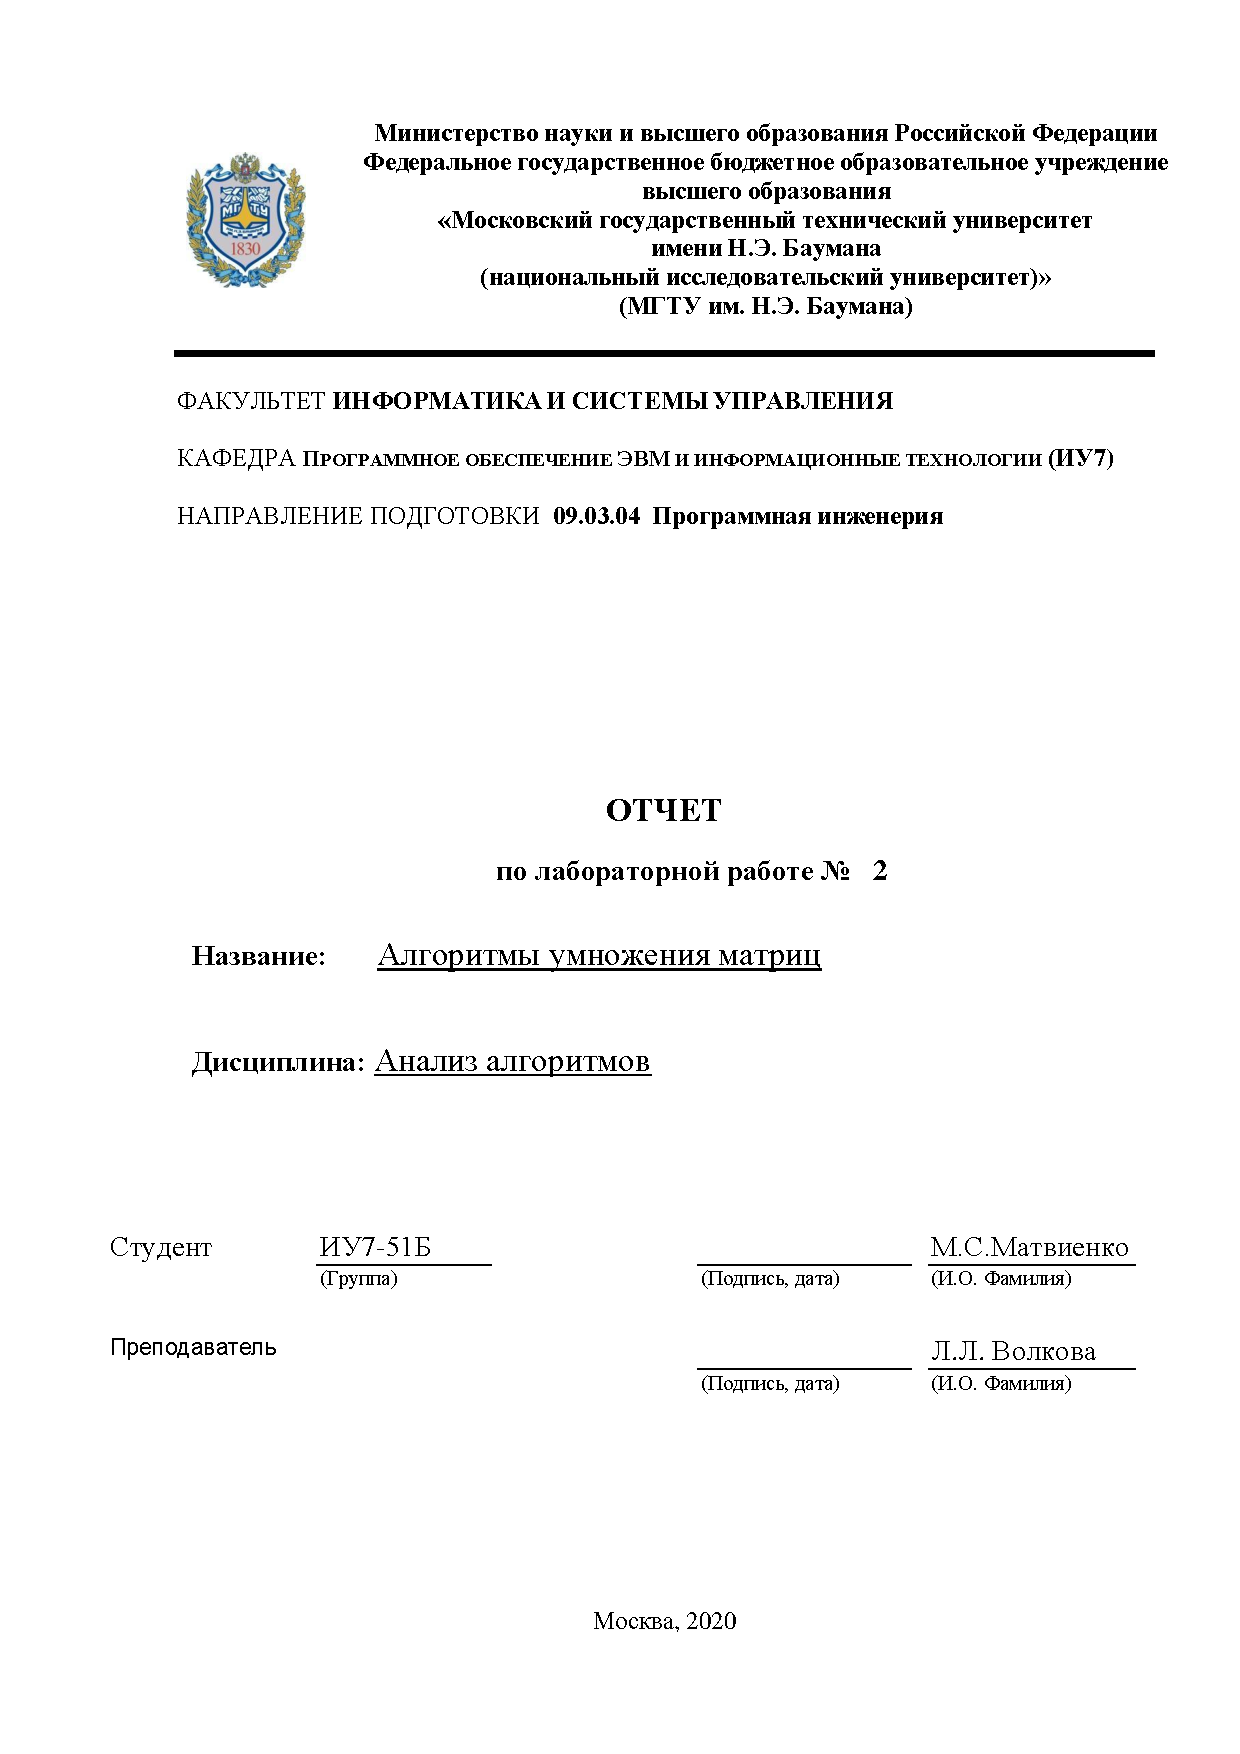
\includegraphics{title_02}
		\end{textblock*}
	\end{titlepage}
\hspace{0pt}
\clearpage

\tableofcontents
\clearpage

\addcontentsline{toc}{section}{Введение}
%//////////////////////////////////////////////////////////////////
\section*{\Huge Введение}
Цель работы: изучение алгоритмов умножения матриц. В данной лабораторной работе рассматривается стандартный алгоритм умножения матриц, алгоритм Винограда и модифицированный алгоритм Винограда.  Также требуется изучить рассчет сложности алгоритмов, получить навыки в улучшении алгоритмов.\\
В ходе лабораторной работы предстоит:
\begin{itemize}
	\item изучить алгоритмы умножения матриц: стандартный и алгоритм Винограда; 
	\item оптимизировать алгоритм Винограда; 
	\item дать теоретическую оценку базового алгоритма умножения матриц, алгоритма Винограда и улучшенного алгоритма Винограда;
	\item реализовать три алгоритма умножения матриц на одном из языков программирования;  
	\item сравнить алгоритмы умножения матриц.
\end{itemize}
\clearpage

\section{Аналитическая часть}
Матрицей A размера $[m*n]$ называется прямоугольная таблица
чисел, функций или алгебраических выражений, содержащая m строк и n столбцов. Числа m и n определяют размер матрицы. Если число столбцов в первой матрице совпадает с числом строк во второй, то эти две матрицы можно перемножить. У произведения будет столько же строк, сколько в первой матрице, и столько же столбцов, сколько во второй.
	    
Пусть даны две прямоугольные матрицы А и В размеров $[m * n]$ и $[n * k]$ соответственно.  
В результате произведение матриц A и B получим матрицу C размера $[m *  k]$.


$c_{i,j} = \sum\limits_{r=1}^n a_{i,r}\cdot b_{r,j}$ называется произведением матриц A и B.

\newpage
\subsection{Описание алгоритмов}

\subsubsection{Стандартный алгоритм}
По определению каждый элемент матрицы C вычисляется следующим образом:\\
$c_{i,j} = \sum\limits_{r=1}^n a_{i,r}\cdot b_{r,j}$, это значит, что для вычисления всей матрицы необходимо выполнить $m *  k$ вычислений, где $(i=1,...,k; j=1,...,m)$

\subsubsection{Алгоритм Винограда}
Подход Алгоритма Винограда является иллюстрацией общей методологии, начатой в 1979-х годах на основе
билинейных и трилинейных форм, благодаря которым большинство усовершенствований для умножения матриц были получены.

Рассмотрим два вектора $V = (v1, v2, v3, v4)$ и $W = (w1, w2, w3, w4)$.  

Их скалярное произведение равно (\ref{formula}) 

\begin{equation} \label{formula}
V \cdot W=v_1 \cdot w_1 + v_2 \cdot w_2 + v_3 \cdot w_3 + v_4 \cdot w_4
\end{equation}

Равенство (\ref{formula}) можно переписать в виде (\ref{formula2}) 
\begin{equation} \label{formula2}
V \cdot W=(v_1 + w_2) \cdot (v_2 + w_1) + (v_3 + w_4) \cdot (v_4 + w_3) - v_1 \cdot v_2 - v_3 \cdot v_4 - w_1 \cdot w_2 - w_3 \cdot w_4
\end{equation}

Менее очевидно, что выражение в правой части последнего равенства допускает предварительную обработку: его части можно вычислить заранее и запомнить для каждой строки первой матрицы и для каждого столбца второй. 
Это означает, что над предварительно обработанными элементами нам придется выполнять лишь первые два умножения и последующие пять сложений, а также дополнительно два сложения.

\subsection{Вывод}
Были рассмотрены алгоритмы классического умножения матриц и алгоритм Винограда, основное отличие которых — наличие предварительной обработки, а также количество операций умножения.
\clearpage

\section{Конструкторская часть}
\textbf{Требования к вводу:}\\
1) На вход подаются две матрицы;\\
\textbf{Требования к программе:}:\\
1) Корректное умножение двух матриц;\\
2) При матрицах неправилыных размеров программа не должна аварийно завершаться;\\
\clearpage
\subsection{Разработка алгоритмов} % Сюда схемы алгоритмов
В данном разделе представлены схемы реализуемых алгоритмов.
\subsubsection{Cтандартное умножения матриц}
\begin{figure}[!htbp]
\centering
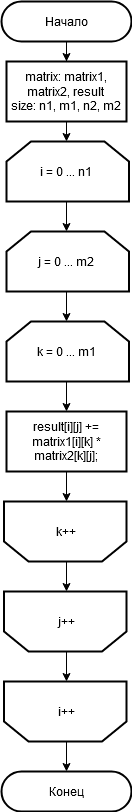
\includegraphics[scale=0.7]{standart}
\caption{Схема классического алгоритма умножения матриц}
\label{fig:mpr}
\end{figure}
\clearpage
\subsubsection{Алгоритм Винограда}
\begin{figure}[!htbp]
\centering
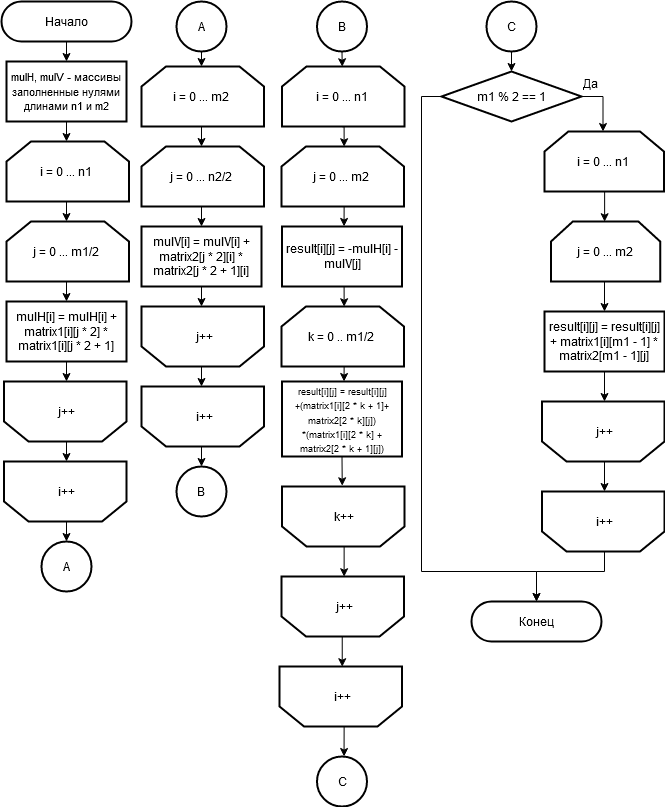
\includegraphics[scale=0.7]{Grape)}
\caption{Схема алгоритма Винограда}
\label{fig:mpr}
\end{figure}
\clearpage
\subsubsection{Оптимизированный алгоритм Винограда}
\begin{figure}[!htbp]
\centering
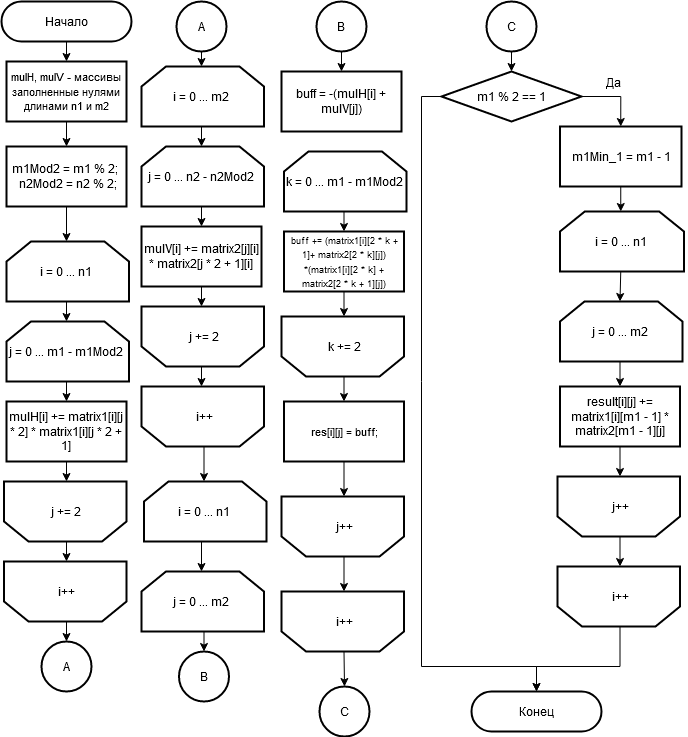
\includegraphics[scale=0.9]{GrapeOpt)}
\caption{Схема оптимизированного алгоритма Винограда}
\label{fig:mpr}
\end{figure}
\clearpage
\subsection{Трудоемкость алгоритмов}
Введем модель трудоемкости для оценки алгоритмов:
\begin{itemize}
	\item базовые операции стоимостью 1 — +, -, *, /, =, ==, <=, >=, !=, +=, [], получение полей класса
	\item оценка трудоемкости цикла: Fц = init +  N*(a + Fтела + post), где a - условие цикла, init - предусловие цикла, post - постусловие цикла
	\item стоимость условного перехода применим за 0, стоимость вычисления условия остаётся
\end{itemize}

Оценим трудоемкость алгоритмов по коду программы.

\subsubsection{Трудоемкость первичной проверки}
Рассмотрим трудоемкость первичной проверки на возможность умножения матриц.

\begin{center}
Табл. 1: Построчная оценка веса\\
	\begin{tabular}{|l c|} 
 	\hline
	Код & Вес \\ [0.5ex] 
 	\hline\hline
 	 int n1 = mart1.Length; & 2\\
 	\hline
	int n2 = matr2.Length; & 2\\
	\hline
	 if (n1  == 0 || n2 == 0) return null; & 3\\
	\hline
	int m1 = mart1[0].Length; & 3\\
	\hline
	int m2 = matr2[0].Length; & 3\\
	\hline
	if (m1 != n2) return null; & 1\\
	\hline\hline
	Итого & 14\\
	\hline
	\end{tabular}
\end{center}

\subsubsection{Классический алгоритм}
Рассмотрим трудоемкость классического алгоритма:  

Инициализация матрицы результата: $2 + 2 + n_1(1 + 3 + 1) = 5n_1 + 4$ 

Подсчет:\\
$1 + n_1(1 + (1 + m_2(1 + (1 + m_1(1 + (8) + 1) + 1) + 1) + 1) + 1) + 1 = 
n_1(m_2(10m_1 + 4) + 4) + 4) + 2 = 10n_1m_2m_1+ 4n_1m_2 + 4n_1 +2
$

\subsubsection{Алгоритм Винограда}
Аналогично рассмотрим трудоемкость алгоритма Винограда.  \\

Первый цикл: $\frac{15}{2}n_1m_1 + 5n_1 + 2$ 

Второй цикл: $\frac{15}{2}m_2n_2+ 5m_2 + 2$

Третий цикл: $13n_1m_2m_1 + 12n_1m_2 + 4n_1 + 2$

Условный переход: $\begin{bmatrix}
             2    &&, \text{невыполнение условия}\\
             15n_1m_2 + 4n_1 + 2 &&, \text{выполнение условия}\\
           \end{bmatrix} $ \\

Итого: $  13n_1m_2m_1 + \frac{15}{2}n_1m_1 +\frac{15}{2}m_2n_2 + 12n_1m_2 + 5n_1 + 5m_2 + 4n_1 + 6 + \\
       \begin{bmatrix}
             2    &&, \text{невыполнение условия}\\
             15n_1m_2 + 4n_1 + 2 &&, \text{выполнение условия}\\
           \end{bmatrix} $ \\

\subsubsection{Оптимизированный алгоритм Винограда}

Аналогично Рассмотрим трудоемкость оптимизированого алгоритма Винограда:\\

Первый цикл: $\frac{11}{2}n_1m_1 + 4n_1 + 2$ 

Второй цикл: $\frac{11}{2}m_2n_2+ 4m_2 + 2$

Третий цикл: $\frac{17}{2}n_1m_2m_1 + 9n_1m_2 + 4n_1 + 2$

Условный переход: $\begin{bmatrix}
             1    &&, \text{невыполнение условия}\\
             10n_1m_2 + 4n_1 + 2 &&, \text{выполнение условия}\\
           \end{bmatrix} $ \\

Итого: $\frac{17}{2}n_1m_2m_1 + \frac{11}{2}n_1m_1 + \frac{11}{2}m_2n_2 + 9n_1m_2 + 8n_1 + 4m_2 + 6 + \\
       \begin{bmatrix}
             1    &&, \text{невыполнение условия}\\
             10n_1m_2 + 4n_1 + 2 &&, \text{выполнение условия}\\
           \end{bmatrix} $ \\

\subsection{Вывод}
В данном разделе были рассмотрены схемы алгоритмов умножения матриц, введена модель оценки трудоемкости алгоритма, были расчитаны трудоемкости алгоритмов в соответсвии с этой моделью.
\clearpage


\section{Технологическая часть}
В данном разделе будет описана технологическая часть лабораторной работы: листинг кода, сравнительный анализ всех алгоритмов.\\
Среда выполнения: Windows 10 x64
\subsection{Средства реализации}
Для выполнения данной лабораторной работы использовался ЯП C\# и IDE VisualStudio \\
Время работы алгоритмов было замерено с помощью класса Stopwatch.
\subsection{Листинг кода}
В данном разделе будет представлен листинг кода разработанных алгоритмов.\\

\subsubsection{Стандартный алгоритм умножения матриц}
\begin{flushleft}
	Листинг 1: Стандартный алгоритм умножения матриц
	\lstinputlisting[language=C]{standart.cs}
\end{flushleft}
\clearpage

\subsubsection{Алгоритм Винограда}
\begin{flushleft}
	Листинг 2: Алгоритм Винограда
	\lstinputlisting[language=C]{Grape).cs}
\end{flushleft}

\subsubsection{Оптимизированный алгоритм Винограда}
\begin{flushleft}
	Листинг 3: Оптимизированный алгоритм Винограда
	\lstinputlisting[language=C]{GrapeOpt).cs}
\end{flushleft}
\clearpage

\subsubsection{Оптимизация алгоритма Винограда}
В рамках данной лабораторной работы было предложено 3 оптимизации:
\begin{enumerate}
	\item Избавление от деления в условии цикла;
	\item Замена $mulH[i] = mulH[i] + …$ на $mulH[i] += …$ (аналогично для $mulV[i]$);
\begin{flushleft}
	Листинг 4: Оптимизация алгоритма Винограда №1 и №2
	\lstinputlisting[language=C]{GrapeOpt12.cs}
\end{flushleft}

	\item Накопление результата в буфер, чтобы не обращаться каждый раз к одной и той же ячейке памяти. Сброс буфера в ячейку матрицы после цикла.
\begin{flushleft}
	Листинг 5: Оптимизации алгоритма Винограда №3
	\lstinputlisting[language=C]{GrapeOpt3.cs}
\end{flushleft}
\end{enumerate}

\subsection{Вывод}
В данном разделе были рассмотрена структура ПО и листинги кода программы.
\clearpage

\section{Исследовательская часть}
\subsection{Сравнительный анализ на основе замеров времени работы алгоритмов}
Был проведен замер времени работы каждого из алгоритмов.\\
Первый эксперимент производится для лучшего случая на квадратных матрицах размером от 100 x 100 до 1000 x 1000 c шагом (100; 100).\\
Сравним результаты для разных алгоритмов:

\begin{center}
\begin{tikzpicture}
\begin{axis}[
    	axis lines = left,
    	xlabel = {Размер матрицы},
    	ylabel = {Время (тики)},
	legend pos=north west,
	ymajorgrids=true
]
\addplot[color=red, mark=square] table[x index=0, y index= 1] {standart0.txt}; 
\addplot[color=green, mark=square] table[x index=0, y index= 1] {Grape0.txt}; 
\addplot[color=blue, mark=square] table[x index=0, y index= 1] {GrapeOpt0.txt}; 

\addlegendentry{Стандартный}
\addlegendentry{Винограда}
\addlegendentry{Опт. Винограда}
\end{axis}
\end{tikzpicture}
\end{center}
\begin{center}
Pис. 4: Сравнение времени работы алгоритмов при четном размере матрицы
\end{center}

Второй эксперимент производится для худшего случая, когда поданы квадратные матрицы с нечетными размерами от 101 x 101 до 1001 x 1001 c шагом (100; 100). 
Сравним результаты для разных алгоритмов:

\begin{center}
\begin{tikzpicture}
\begin{axis}[
    	axis lines = left,
    	xlabel = {Размер матрицы},
    	ylabel = {Время (тики)},
	legend pos=north west,
	ymajorgrids=true
]
\addplot[color=red, mark=square] table[x index=0, y index= 1] {standart1.txt}; 
\addplot[color=green, mark=square] table[x index=0, y index= 1] {Grape1.txt}; 
\addplot[color=blue, mark=square] table[x index=0, y index= 1] {GrapeOpt1.txt}; 

\addlegendentry{Стандартный}
\addlegendentry{Винограда}
\addlegendentry{Опт. Винограда.}
\end{axis}
\end{tikzpicture}
\end{center}
\begin{center}
Pис. 5: Сравнение времени работы алгоритмов при нечетном размере матрицы
\end{center}

\subsection{Тестирование программы}
Было произведено тестирование реализованных алгоритмов с помощью библиотеки 
Microsoft.VisualStudio.TestTools.UnitTesting.\\
Всего было реализованно 7 тестовых случаев:
\begin{itemize}
	\item Некорректный размер матриц. Алгоритм должен возвращать Null
	\item Размер матриц равен 1
	\item Размер матриц равен 2
	\item Сравнение работы стандартной реализации с Виноградом на случайных значениях
	\subitem Четный размер
	\subitem Нечетный размер
	\item Сравнение работы стандартной реализации с оптимизированным Виноградом на случайных значениях
	\subitem Четный размер
	\subitem Нечетный размер
\end{itemize}

На рисунке \ref{fig:test} будут предоставлены результаты тестирования программы. Откуда видно, что тестирование пройдено, алгоритмы реализованы правильно.
\begin{figure}[!htbp]
\centering
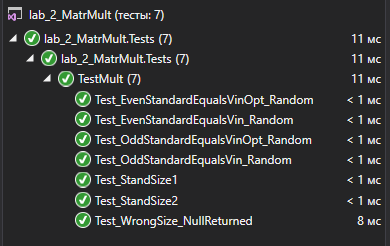
\includegraphics[scale=0.9]{TestsPassed}
\caption{Результаты работы тестов}
\label{fig:test}
\end{figure} 

\subsection{Вывод}
По результатам тестирования все рассматриваемые алгоритмы реализованы правильно. Самым медленным алгоритмом оказался алгоритм классического умножения матриц, а самым быстрым — оптимизированный алгоритм Винограда.

\clearpage
\addcontentsline{toc}{section}{Заключение}
%//////////////////////////////////////////////////////////////////
\section*{\Huge Заключение}
В ходе лабораторной работы я изучил алгоритмы умножения матриц: стандартный и Винограда, оптимизировал алгоритм Винограда, дал теоретическую оценку алгоритмов стандартного умножения матриц, Винограда и улучшенного Винограда, реализовал три алгоритма умножения матриц на языке программирования C\# и сравнил эти алгоритмы.
\end{document}